\usepackage{../pvm}

\usetikzlibrary{shadows,shapes.multipart}

\title{Smart Pointers}
\author{Fr\'ed\'eric Vogels}


\begin{document}

\begin{frame}
  \titlepage
\end{frame}

\begin{frame}
  \frametitle{RAII}
  \begin{itemize}
    \item RAII: resource management
    \item Destructor is in charge of cleanup
    \item No resource leaks anymore
    \item Examples: {\tt ifstream} for reading files, {\tt vector}, \dots
    \item What about heap allocated memory?
  \end{itemize}
\end{frame}

\begin{frame}
  \frametitle{Heap Allocation}
  \code[font size=\small]{heap-allocation.cpp}
  \begin{procontralist}
    \con Memory leak
  \end{procontralist}
\end{frame}

\begin{frame}
  \frametitle{Heap Allocation}
  \code[font size=\small]{delete-person.cpp}
  \begin{procontralist}
    \pro Memory gets deleted if all goes well
    \con Memory leak in case of exceptions
    \con Easy to forget {\tt delete}
    \con Fragile if multiple exit points (e.g. {\tt return}, {\tt throw})
  \end{procontralist}
\end{frame}

\begin{frame}
  \frametitle{Heap Allocation}
  \code[font size=\small]{person-deleter.cpp}
  \begin{procontralist}
    \pro Memory guaranteed to be freed
    \con Need to remember to always use {\tt Person\_deleter}
    \con {\tt Person\_deleter} works only on {\tt Person}s
  \end{procontralist}
\end{frame}

\begin{frame}
  \frametitle{Heap Allocation}
  \code[font size=\small]{deleter.cpp}
  \begin{procontralist}
    \pro Memory guaranteed to be freed
    \pro {\tt deleter} usable on all types
    \con Need to remember to always use {\tt deleter}
  \end{procontralist}
\end{frame}

\begin{frame}
  \frametitle{Heap Allocation}
  \code[font size=\small,width=.9\linewidth]{smart_pointer.cpp}
  \begin{procontralist}
    \pro Memory guaranteed to be freed
    \pro {\tt smart\_pointer} usable on all types
    \con Clumsy syntax to access members: {\tt p.get()->member}
  \end{procontralist}
\end{frame}

\begin{frame}
  \frametitle{Solving The Syntax Issue}
  \code[font size=\small]{smart_pointer2.cpp}
  \begin{itemize}
    \item We want {\tt p} to look as much like a regular pointer as possible
  \end{itemize}
\end{frame}

\begin{frame}
  \frametitle{Solving The Syntax Issue}
  \code[font size=\small]{overload-member-access.cpp}
  \begin{itemize}
    \item Overloading {\tt ->} operator is possible
  \end{itemize}
\end{frame}

\begin{frame}
  \frametitle{Dereferencing Smart Pointers}
  \begin{itemize}
    \item Dereferencing: given pointer {T* p}, get pointee using {\tt *p}
    \item We want to be able to use {\tt *p} on smart pointers too
    \item Again, we want smart pointers to behave the same as regular pointers
  \end{itemize}
  \code{dereferencing.cpp}
\end{frame}

\begin{frame}
  \frametitle{Dereferencing Smart Pointers}
  \code[font size=\small]{overload-dereference.cpp}
  \begin{itemize}
    \item Overloading {\tt ->} operator is possible
  \end{itemize}
\end{frame}

\begin{frame}
  \frametitle{Dumb Pointers vs Smart Pointers}
  \begin{itemize}
    \item Dumb pointer {\tt T*}
    \item Smart pointer {\tt smart\_ptr<T>}
    \item Smart pointers should automatically {\tt delete} themselves when necessary
          \begin{itemize}
            \item Achieved using destructor
          \end{itemize}
    \item Same syntax for dumb as for smart pointers
          \begin{itemize}
            \item Achieved using operator overloading
            \item Operators {\tt ->}, {\tt *}, {\tt []}, etc.
          \end{itemize}
  \end{itemize}
\end{frame}

\begin{frame}
  \frametitle{Problem}
  \code[font size=\small,width=.9\linewidth]{duplication.cpp}
  \begin{enumerate}
    \item We create a new person {\tt q}, aged 20
    \item We call {\tt make\_older}, passing the smart pointer by value.
    \item {\tt make\_older} increases the age
    \item {\tt p} goes out of scope, and it {\tt delete}s the {\tt Person}
    \item We try to print {\tt q}'s age, but {\tt q} points to invalid memory
  \end{enumerate}
\end{frame}

\begin{frame}
  \frametitle{Problem}
  \begin{center}
    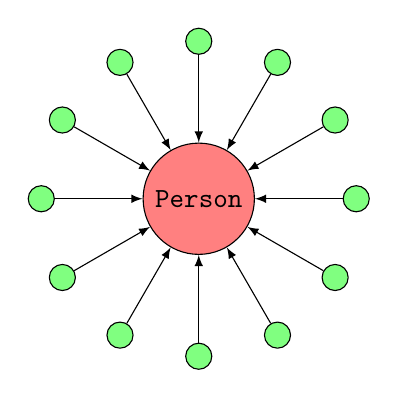
\begin{tikzpicture}[object/.style={draw,circle,fill=red!50},
                        pointer/.style={draw,circle,fill=green!50,font=\tiny}]
      \node[object] (person) at (0,0) {\tt Person};

      \foreach \a in {0,30,...,330} {
        \node[pointer] (ptr) at (\a:2cm) {};
        \draw[-latex] (ptr) -- (person);
      }
    \end{tikzpicture}
  \end{center}
  \begin{itemize}
    \item When copying smart pointers, they point to the same object
    \item When one smart pointer dies, it will {\tt delete} the object.
    \item All other pointers become invalidated.      
  \end{itemize}
\end{frame}

\begin{frame}
  \frametitle{Ownership}
  \begin{itemize}
    \item Ownership: you're responsible for freeing the object
    \item No ownership: you're forbidden to free the object
    \item A {\tt smart\_ptr} has ownership
    \item We use {\tt T*} to indicate no ownership
    \item Problem with previous code: we had two smart pointers, hence two owners, which is bad
  \end{itemize}
\end{frame}

\begin{frame}
  \frametitle{Fix to the Problem}
  \code[font size=\small,width=.9\linewidth]{duplication2.cpp}
\end{frame}

\begin{frame}
  \frametitle{Prohibiting Multiple Ownership}
  \begin{itemize}
    \item For every object, we want exactly one owner
    \item We need to prohibit copying smart pointers
  \end{itemize}
  \code[font size=\small,width=.9\linewidth]{prohibiting-copies.cpp}
\end{frame}

\begin{frame}
  \frametitle{Prohibiting Multiple Ownership}
  \begin{itemize}
    \item Remove copy constructor
    \item Remove assignment operator
  \end{itemize}
  \code[font size=\small,width=.9\linewidth]{prohibiting-copies-solution.cpp}
\end{frame}

\begin{frame}
  \frametitle{Transferring Ownership}
  \begin{itemize}
    \item Sometimes we do want to transfer ownership
    \item Possible to write {\tt transfer} function
    \item Technical details not important (\link{http://thbecker.net/articles/rvalue_references/section_01.html}{r-value references})
  \end{itemize}
  \code[font size=\small]{transfer.cpp}
\end{frame}

\begin{frame}
  \frametitle{Transferring Ownership: Example}
  \code[font size=\small,width=.9\linewidth]{transfer-example.cpp}
\end{frame}

\begin{frame}
  \frametitle{\tt std::unique\_ptr}
  \structure{Pre \cpp11}
  \begin{itemize}
    \item Make your own {\tt smart\_pointer}
    \item Or rely on external library (e.g.~Boost)
  \end{itemize}
  \vskip5mm
  \structure{Since \cpp11}
  \begin{itemize}
    \item Present in \cpp's standard library
    \item Named {\tt std::unique\_ptr}
    \item Creation: {\tt std::make\_unique<T>(args)}
    \item Transferring: {\tt q = std::move(p)}
    \item {\tt \#include <memory>}
  \end{itemize}
\end{frame}

\begin{frame}
  \frametitle{{\tt std::unique\_ptr} Example}
  \code[font size=\small,width=.95\linewidth]{unique-ptr-example.cpp}
\end{frame}

\begin{frame}
  \frametitle{The Magic of {\tt std::make\_unique<T>}}
  \begin{itemize}
    \item {\tt std::make\_unique<T>} can take the same arguments as {\tt T}'s constructors
  \end{itemize}
  \code[font size=\small]{magic-make-unique.cpp}
\end{frame}

\begin{frame}
  \frametitle{Problems With Single Ownership}
  \begin{itemize}
    \item Say you have an object O
    \item Say many other objects need access to O
    \item Who should have ownership?
  \end{itemize}
  \begin{center}
    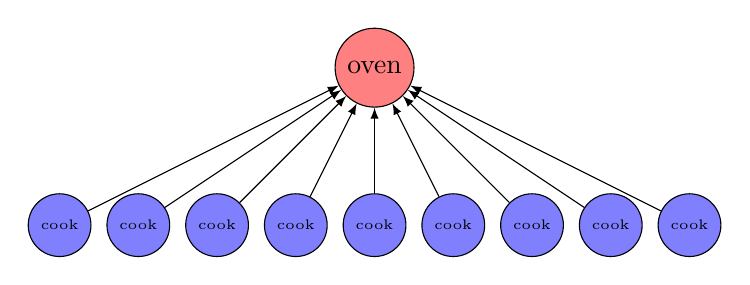
\begin{tikzpicture}[utensil/.style={draw,fill=red!50,circle},
                        cook/.style={draw,fill=blue!50,circle,font=\tiny}]
      \node[utensil] (utensil) at (0,0) {oven};
      
      \foreach \x in {-4,...,4} {
        \node[cook] (cook) at (\x, -2) {cook};
        \draw[-latex] (cook) -- (utensil);
      }
    \end{tikzpicture}
  \end{center}
\end{frame}

\begin{frame}
  \frametitle{Attempts at Solutions}
  \structure{Proposal}
  \begin{itemize}
    \item Give one cook ownership?
    \item This cook takes oven with him to his grave
    \item We have to make sure the oven owning cook dies last
    \item Otherwise, all other cooks would be using a phantom oven
  \end{itemize}
  \vskip5mm
  \structure{Critique}
  \begin{itemize}
    \item Solution seems quite arbitrary
    \item Fragile
  \end{itemize}
\end{frame}

\begin{frame}
  \frametitle{Attempts at Solutions}
  \structure{Proposal}
  \begin{itemize}
    \item Introduce new object {\tt Kitchen}
    \item Kitchen owns oven and cooks
    \item Kitchen has to survive cooks and oven
  \end{itemize}
  \vskip5mm
  \structure{Critique}
  \begin{itemize}
    \item Structured
    \item Relatively robust
    \item Absolute need to keep kitchen alive
  \end{itemize}
\end{frame}

\begin{frame}
  \frametitle{Attempts at Solutions}
  \structure{Proposal}
  \begin{itemize}
    \item Introduce shared ownership
    \item Each cook owns oven
    \item Oven keeps track of number of ovens
    \item New cook increments count
    \item Dead cook decrements count
    \item When no cooks left, oven self destructs
  \end{itemize}
  \vskip5mm
  \structure{Critique}
  \begin{itemize}
    \item Structured
    \item Robust
    \item (There are shortcomings, but we'll ignore them)
  \end{itemize}
\end{frame}

\begin{frame}
  \frametitle{\tt shared\_ptr}
  \begin{itemize}
    \item Standard library offers ready made solution
    \item {\tt shared\_ptr<T>}
    \item Creation: {\tt make\_shared<T>(args)}
    \item No ownership transfer necessary
    \item When shared ptr is duplicated, reference count goes up
    \item When shared ptr goes out of scope, refcount goes down
    \item When refcount reaches 0, memory is freed
    \item We'll be using this pointer most from now on
    \item No more {\tt T*}
  \end{itemize}
\end{frame}

\end{document}


%%% Local Variables:
%%% mode: latex
%%% TeX-master: "smart-pointers"
%%% End:
